\documentclass[25pt, a0paper,
               colspace=15mm, subcolspace=0mm,
               blockverticalspace=17mm, margin=1in, total={35in, 44in},
               landscape]{tikzposter} % See Section 

\usepackage{poster}
\usepackage{array}
\usepackage{multirow}
\usepackage{multicol}
%\usepackage[table,xcdraw]{xcolor}

\definecolor{PaleBlue}{rgb}{0,.55,.9}
\definecolor{PaleGreen}{rgb}{0,.7,.25}
\definecolor{RedPink}{rgb}{.9,0,.2}
\definecolor{Pink}{rgb}{.85,.35,.7}
\definecolor{Purple}{rgb}{.6,0,.75}
\definecolor{Orange}{rgb}{.9,.3,.05}

\colorlet{attentionColor}{Orange}
\colorlet{charEmbedColor}{RedPink}
\colorlet{predEmbedColor}{Pink}
% \colorlet{attentionColor}{GoldUL!90!black}
% \definecolor{attentionColor}{rgb}{.85,.5,.6}



\def\pathwidth{2pt}
\def\nodewidth{3pt}
\def\cornerCurvature{7pt}

\tikzstyle{embed}=[%
  draw,
  #1,
  % line width=3pt,
  anchor=north,
  minimum width=.8cm,
  minimum height=1.6cm,
  inner sep=0pt,
  text=#1!65!black,
  font=\fontsize{25pt}{24}\selectfont,
  ]

\title{\parbox{\linewidth}{\centering Exploring Pruning Filters In Convolution Neural Network}}
\institute{Department of Computer Science and Software Engineering, Université Laval}
\author{Vincent Martineau}

\begin{document}
\maketitle

\begin{columns}
\column{.4}
\block{Introduction}{%
We explore how reducing network expressivity can affect performance in Convolution Neural Network (CNN). The idea is to take a network that can handle a more complex task and remove filters that are the least important for the new task.

\vspace{5mm}
\textbf{Motivations:}
\begin{itemize}
  \item \colorbold{Reduce} network size and execution time.
  % \item Goldberg (2017) emphasizes this fact for NLP tasks such as part of speech tagging (POS) or named entity recognition (NER).
  \item \colorbold{Run} network on less demanding hardware with similar accuracy.
\end{itemize}

\vspace{15mm}
\textbf{Related work:}
\begin{itemize}
  \item P.Molchanov et al. (2017): Pruning Convolutional Neural Networks for Resource Efficient Inference.
\end{itemize}

\vspace{0mm}
\textbf{Goals:}
\begin{itemize}
  \item Reduce training time to produce sufficient network.
  \item Provide a module that could handle multiple models.
   \item Explore the effect of pruning for speed and size.
\end{itemize}
}

\column{0.30}
\block{Comparing Various Level of Pruning}{

\vspace{-15pt}

\begin{center}
	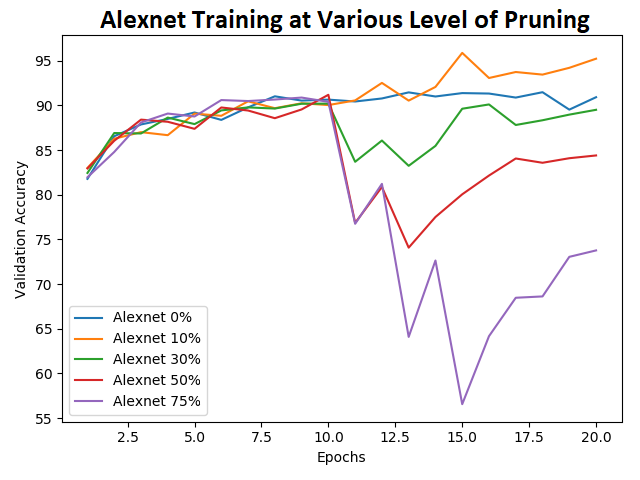
\includegraphics[width=25cm, height=15cm]{figures/prune_ratio}
\end{center}

This graph compare various level of pruning. Each level of pruning is made on two iterations made after 10 epochs of training and 3 epochs or retraining per iteration. Pretrained weight were used to see the impact on transfer learning.
}

\column{0.30}
\block{Comparing Pruning on  Multiple Models}{
	
	\vspace{-15pt}
	
\begin{center}
	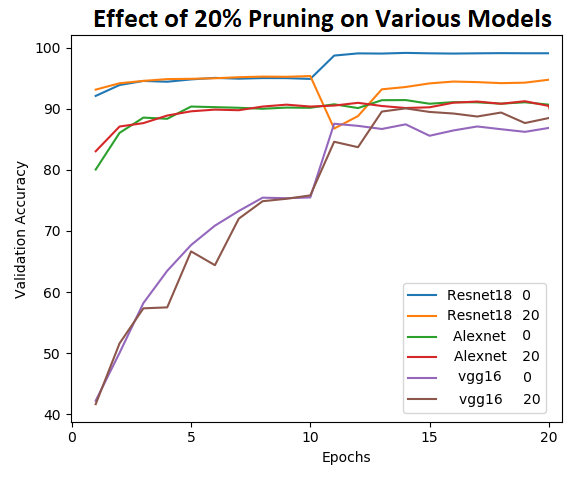
\includegraphics[width=25cm, height=15cm]{figures/various_models}
\end{center}

This graph explore the effect of pruning on different models. Each model shows the effect of pruning 20\% of the convolution filters in one step after 10 epochs of training.
}
\end{columns}

\begin{columns}
\column{0.50}
\block{Example of Network Reduction}{
	
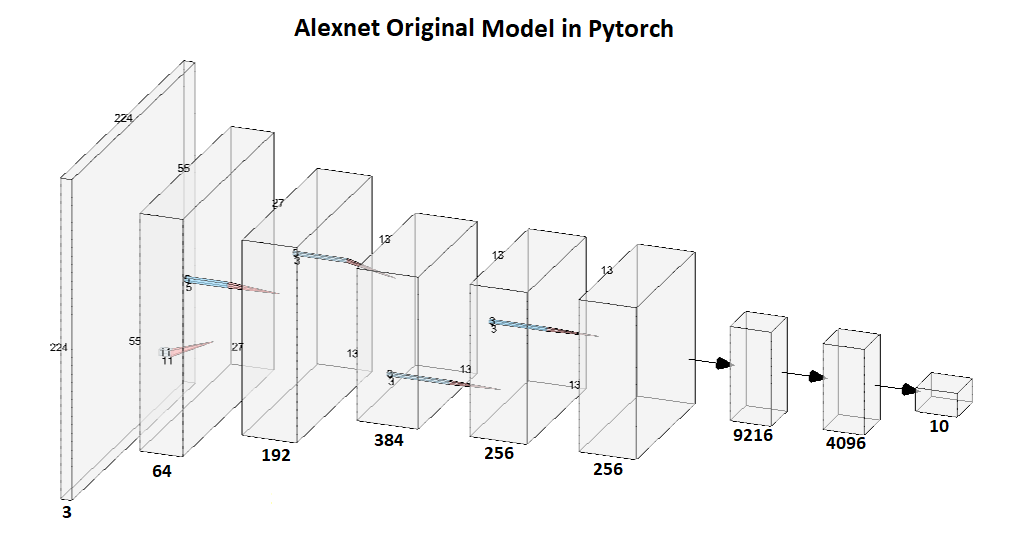
\includegraphics{figures/Alexnet_origin}
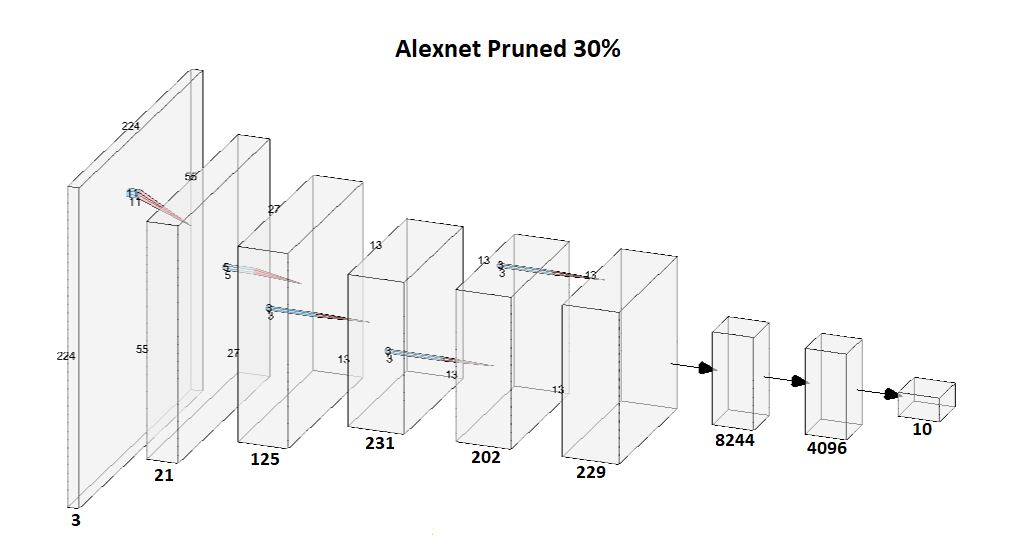
\includegraphics{figures/Alexnet_30}
	
	Comparing the effect of pruning on Alexnet. Left is the original model provided by pytorch. On the right is Alex net pruned 30\%. In the case of network like Alexnet there is an important reduction of parameters based on the reduction of the first fully connected layer. There is also an important reduction in the first layers.
\vspace{41pt}
}


  \column{.25}
  \block{Algorithm}{
  	\begin{itemize}
  	\item Pretrain network with full paramters
  	\item \textbf{Prepare Pruning}
  	\begin{itemize}
  	\item Convert model to ONNX
  	\item Extract execution graph
  	\item Determine which layer can be pruned
    \end{itemize}
  	\item \textbf{Prune network}
  	\begin{itemize}
  		\item Find number of filter to prune on iteration
  		\item Wort filter based on activation mean
  		\item Remove filters
  		\item Apply pruning effect to next layers
  		\item Reset optimizer
  	\end{itemize}
  	\item Finalize training
  \end{itemize}
  }

  \column{.25}
\block{Settings}{
	\begin{itemize}
		\item \textbf{Dataset}: Cifar10
		\item \textbf{Optimizer}: Stochastic Gradient Descent
		\item \textbf{Learning Rate}: 0.01
		\item \textbf{Momentum}: 0.0
		\item \textbf{Nesterov}: False
		\item \textbf{Batch Size}: 64
		\item \textbf{Use GPU}: Yes
	\end{itemize}
\textbf{Pruning:}
\begin{itemize}
	\item \textbf{Pretrain Epoch}:  10
	\item \textbf{Retrain Epoch}: 3
	\item \textbf{Total nb. Epoch}: 20
\end{itemize}
\item \textbf{Nb Iteration on Alexnet}:  2
\item \textbf{Nb Iteration on Model Compare}:  1
\vspace{-4pt}
}

\end{columns}


\begin{columns}

  \column{.3}
  \block{Performances}{
  % \vspace{3mm}
\begin{center}
	\textbf{Comparing Alexnet Attributes After Pruning}
\begin{tabular}{c|c|cc|cc|cc|cc}
	& \textbf{0\%} & \multicolumn{2}{c|}{\textbf{10\%}}       & \multicolumn{2}{c|}{\textbf{30\%}}       & \multicolumn{2}{c|}{\textbf{50\%}}       & \multicolumn{2}{c}{\textbf{75\%}}        \\ \hline
	\textbf{FLOPs(G)}  & 0.815        & 0.665 & {\color[HTML]{009901} (-18.4\%)} & 0.445 & {\color[HTML]{009901} (-45.3\%)} & 0.283 & {\color[HTML]{009901} (-65.3\%)} & 0.133 & {\color[HTML]{009901} (-83.7\%)} \\ \hline
	\textbf{Params(M)} & 57.0         & 54.8  & {\color[HTML]{009901} (-3.86\%)} & 47.3  & {\color[HTML]{009901} (-17.0\%)} & 37.6  & {\color[HTML]{009901} (-34.0\%)} & 27.0  & {\color[HTML]{009901} (-52.6\%)}             
\end{tabular}
\end{center}
\begin{center}
	\textbf{Comparing Pruning On Various Models}
	\begin{tabular}{llllllllll}
		\textbf{}                               & \multicolumn{3}{c}{\textbf{VGG}}                                                                         & \multicolumn{3}{c}{\textbf{Alexnet}}                                                                     & \multicolumn{3}{c}{\textbf{Resnet18}}                                               \\
		& \multicolumn{1}{c}{0\%} & \multicolumn{1}{c}{20\%} & \multicolumn{1}{c}{Diff}                            & \multicolumn{1}{c}{0\%} & \multicolumn{1}{c}{20\%} & \multicolumn{1}{c}{Diff}                            & \multicolumn{1}{c}{0\%} & \multicolumn{1}{c}{20\%} & \multicolumn{1}{c}{Diff}       \\ \cline{2-10} 
		\multicolumn{1}{c|}{\textbf{FLOPs(G)}}  & 17.31                   & 12.23                    & \multicolumn{1}{l|}{{\color[HTML]{009901} -29.3\%}} & 0.815                   & 0.592                    & \multicolumn{1}{l|}{{\color[HTML]{009901} -27.3\%}} & 1.83                    & 1.13                     & {\color[HTML]{009901} -38.2\%} \\
		\multicolumn{1}{c|}{\textbf{Params(M)}} & 134.3                   & 103.7                    & \multicolumn{1}{l|}{{\color[HTML]{009901} -22.8\%}} & 57.0                    & 48.2                     & \multicolumn{1}{l|}{{\color[HTML]{009901} -15.4\%}} & 11.18                   & 5.27                     & {\color[HTML]{009901} -52.9\%}
	\end{tabular}
\end{center}

{\tiny element considered in FLOP: Conv1d, Conv2d, Conv3d, ConvTranspose2d, BatchNorm1d, BatchNorm2d, BatchNorm3d, ReLU, ReLU6, LeakyReLU, MaxPool1d, MaxPool2d, MaxPool3d, AdaptiveMaxPool1d, AdaptiveMaxPool2d, AdaptiveMaxPool3d, AvgPool1d, AvgPool2d, AvgPool3d, AdaptiveAvgPool1d, AdaptiveAvgPool2d, AdaptiveAvgPool3d, Linear}
  
  }


  \column{.3}
  \block{Observations}
  {
  	\begin{itemize}
   \item Not all convolutional layer can be pruned. Pruning layers before a residual connection is dangerous because both side of the residual connection must have the same side.
  \item When pruning in a convolution layer it is important to propagate to the following layers so the next layers have the right input size. This apply to convolution, linear and batchnorm layers..
  \item It is been seen that algorith leave only one filter on a layer. When this happen it reduce the quality of the results.
  \item When pruning it is important to reset optimizer.
  \end{itemize}
\vspace{0.5cm}
  }

  \column{.4} 
  \block{Conclusion}{
  \vspace{1.0cm}
  \textbf{Discussion:}
    \begin{itemize}
        \item It is a  \colorbold{possible} to support multiple model type using the same module.
        \item The reduction on some model is \colorbold{impressive} and could be run on lower trier hardware.
    \end{itemize}
    
    \textbf{Future Works:}
    \begin{itemize}
        \item  Pruning proved to be a valid form of regulation.
        \item  Would be possible to use different criteria to sort filters.
        \item  Experiments were made on Cifar10. It would be interesting to try on various datasets.
    \end{itemize}
    \vspace{1.6cm}
  }
\end{columns}

\end{document}
